\documentclass[../main.tex]{subfiles}
\graphicspath{{\subfix{../Images}}}

\begin{document}
\section{Research Plan}
\label{sec:research_plan}
%% RESEARCH PLAN
\subsection{Introduction}
The project presented in this document is the main research idea presented towards the completion of the Doctoral Program of the 38\textsuperscript{th} cycle of the Italian National Program in Doctoral Research - Blockchain and Distributed Ledger Technology in Social Systems and Smart Societies.
\par
I, Ricardo Almeida, graduated in Physics and Chemistry by the University of Evora, and with a Master's in Electronic Engineering and Telecommunications by the University of Aveiro, both universities in Portugal, from where I'm originally from, was awarded a 3 year scholarship towards the execution of a research plan centered on decentralised (blockchain based) electronic voting systems.

\subsection{Doctoral Project Outline}
\label{sec:project_outline}
The idea for this project was inspired by personal curiosity for blockchain technology, which was developed prior to the decision of engaging in the PhD program, and another parallel interest in general governance, but also motivated by the novelty of new technology and the potential for new solutions to existing problems through a novel decentralised approach. Initially this project had a more generalist approach due to the lack of support from blockchains to voting systems. A review of existing blockchain-based e-voting proposals in academia revealed an environment where researchers were trying to discover how to use blockchains developed with financial purposes in mind, namely cryptocurrency-centered blockchains, towards different applications. The introduction of smart contracts by the Ethereum blockchain opened significantly the spectrum of research possibilities, but the most significant breakthrough in this context came with the popularisation and standardisation of Non-Fungible Tokens (NFT).
\par
NFTs provide an interesting new approach to developing a blockchain-based voting systems. NFTs are inherently scarce, indivisible and individually unique. Also, the mechanics that regulate transferring them among users are transparent, since these are always smart contract functions that can be publicly verified, and secure. All NFT operations, from when they are minted until when they are burned, are recorded permanently in the blockchain, which makes NFTs highly traceable. These properties happen to be also highly desirable in a voting ballot. From this observation, the idea of including NFTs to abstract voting ballots in a blockchain-based voting system was quite obvious.
\par
Non-Fungible Tokens are a general idea. From the implementation point of view, the last years saw many public blockchains being introduced with explicit NFT support built in, normally through its support for some sort of smart contract programming paradigm that also supports NFT creation and mechanics. As such, it was evident that the specific technology used in the context of this project would be determinant to any conclusions obtained. In this sense, the doctoral project was expanded to also investigate how significantly different blockchain architectures behave when used to develop a NFT centered voting system and how these differences can influence the intrinsic characteristics of the system itself.
\par
Among the potential choices of blockchains, I'm focused in comparing the most popular of smart contract/NFT supporting blockchains - Ethereum, with Flow \cite{flow2020a}, a blockchain that, incidently, was created specifically to address scalability and interoperability issues that arose from running the \textit{CryptoKitties} project in the Ethereum blockchain. The \textit{CryptoKitties} smart contract created one of the first interactive NFT projects in Ethereum, one whose sudden and unexpected popularity put the throughput limits of the Ethereum network to a test \cite{bbc2017}. The team behind this project tried to overcome the limitations of the Ethereum network, initially by adjusting the Solidity contract, but eventually they decided to create their own blockchain from scratch. Flow was created to the most efficient blockchain to trade NFTs in. Its main difference from Ethereum resides on how these chains store data, specifically, NFT related data. Ethereum uses a \textit{contract-based} storage approach, where all NFT fields are stored on chain with a reference to the minting contract, i.e, the NFT minting contract is the central storage element, while Flow developed a more decentralised, \textit{account-based} storage approach. In Flow, contracts and NFTs are two different data elements and both are saved relative to an \textit{account}, as in a normal blockchain account, akin to the Externally Owned Accounts from Ethereum, rather than a contract address as in Ethereum. Account storage spaces in Flow can only be modifies by the account owner and any external accesses to digital objects in storage must be explicitly given previously by the owner. Flow and Ethereum differ in other aspects, but the method in which data is saved on chain is the most influential for this purpose.
\par
Though both blockchain implement the same construct, they do so in fundamentally different ways. Due to, perhaps, the novelty of the whole context, there are no objective comparisons between these two approaches published academically or otherwise, neither from a generalist point of view, less even from a electronic voting system development perspective, definitely motivation for this project. Ifg. \ref{fig:general_solution} presents a general idea of the approach considered for a NFT based e-voting system.

\begin{figure}[htp]
    \centering
    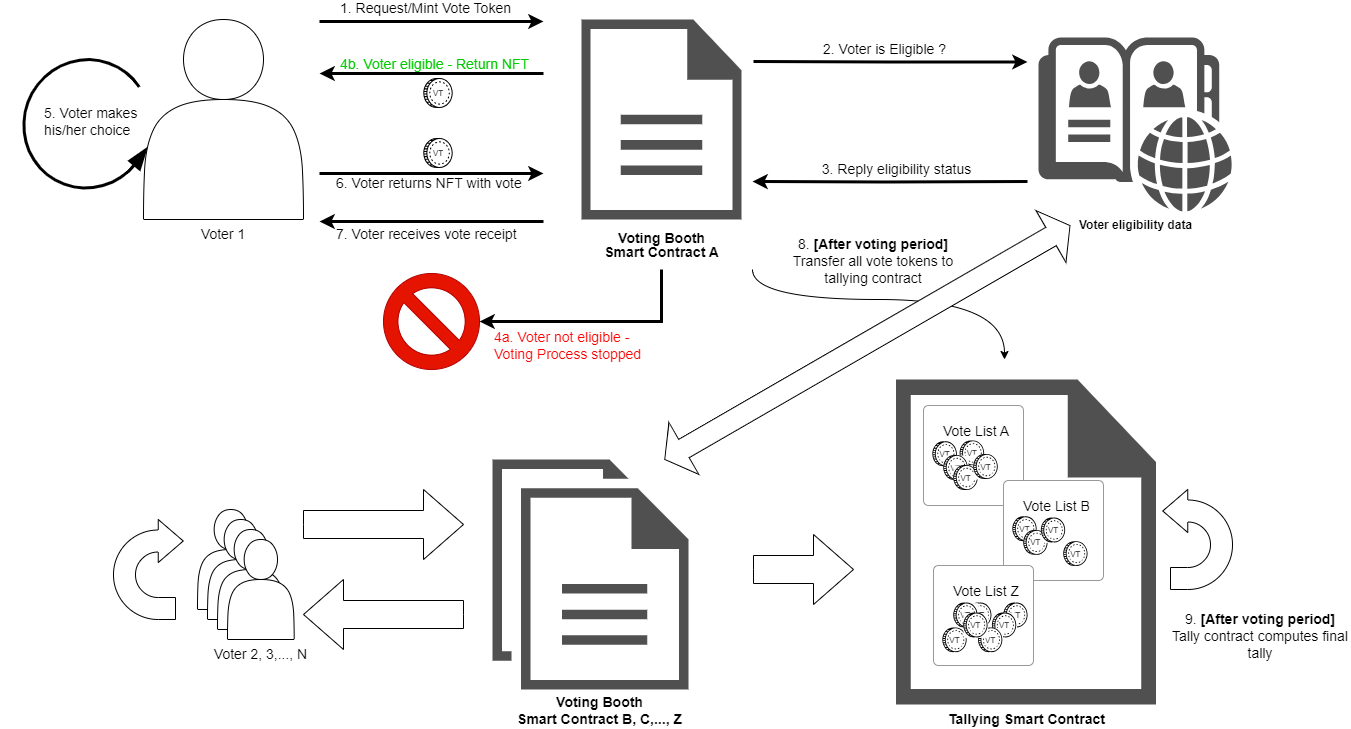
\includegraphics[width=0.7\textwidth]{../Images/01_general_solution.png}
    \caption{General solution adopted to experiment with the different storage architectures considered.}
    \label{fig:general_solution}
\end{figure}

\subsubsection{Collaboration with the University of Surrey}
The Italian \textit{Dottorato di Ricerca di Interesse Nazionale} program establishes a period of 6 months minimum to a maximum of one year where the doctoral research must be undertaken in an foreign (non-Italian) university or research institution. The University of Surrey was chosen to this purpose by several reasons:
\begin{enumerate}
    \item {Similar to the University of Pisa, Surrey maintains a dedicated Blockchain and Distributed Ledger Technology research group, as well as researchers active in electronic voting systems development, something that is not yet common in most European universities.}
    \item {I've collaborated with U. Surrey researchers recently in a research project in a similar area (homomorphic encryption) and the feedback of such collaboration was largely positive.}
    \item {I'm already quite familiar with the United Kingdom, both the country and the culture. I've worked with British organisations and lived in British soil in the past and I have most of my British bureaucratic elements still active, namely a bank account and a valid National Insurance Number which, hopefully, can make a transition back to the UK easier.}
\end{enumerate}

\subsection{Research Questions}
The salient research points indicated in Sec. \ref{sec:project_outline} were summarised in the following set of Research Questions:
\begin{enumerate}
    \item {What advantages, if any, does a \textit{account-based} storage architecture provides when compared with a \textit{contract-based} approach regarding implementing Non-Fungible Token based smart contracts?}
    \item {Can Non-Fungible Tokens be used to develop a secure, transparent and private blockchain-based voting system, using these tokens to abstract the voting ballot?}
    \item {If NFTs are indeed useful to be used in a decentralised e-voting context, which of the storage architectures considered produces the better option?}
\end{enumerate}

% Cadence vs. Ethereum
\subsection{State of the Art/Related Works}
Research in electronic voting systems as been active for several decades now and started parallel to the first breakthroughs in commercial cryptography techniques. Until the 1970s, cryptography was mostly used in a military context, but a landmark article by Diffie and Hellman published in 1976 \cite{Diffie1976} opened the doors to commercial applications, as well as laying the groundwork for most of the research in electronic voting systems that followed it.
\par
This field evolved somewhat linearly over the following 30 years, with new proposals to novel voting systems following the introduction of new commercial cryptographic techniques, such as symmetrical and asymmetrical encryption schemes, digital signatures, hash algorithms, blind signatures, homomorphism, mix-nets, etc. This pace was kept until relatively recently, when another landmark publication changed the research landscape. In 2009, the mysterious Satoshi Nakamoto published a white paper detailing Bitcoin, the first instance of a cryptocurrency, also introducing the blockchain concept was critical for the whole process to work \cite{Nakamoto2008}. Though this publication had no direct relation to the e-voting research, the applicability of blockchain (and cryptocurrencies by extension) in the voting context was obvious. Soon after, the first blockchain-based e-voting proposals came to light, with the rate of new proposals following new blockchain features and tools, such as smart contracts, consensus algorithms and even new architectural approaches, like it was already happening with commercial cryptography.
\par
The main conclusion and results for this exercise were published in a journal article \cite{Almeida2023} at the end of year 1 of this program. Following this exercise, further investigation was undertaken towards determining the extent at which academic publications were focusing either in new blockchain architectures and using these new architectures to improve existing voting systems. Though the shift towards the usage of smart contracts was quite evident in new decentralised proposals, as indicated in \cite{Almeida2023}, so far the same does not seem to apply to Non-Fungible Tokens. Up to the time of this writing, I have not been able to find any academic publications detailing any architectural comparisons between blockchain implementations nor any e-voting proposals where NFTs are used explicitly to establish the voting system.

\subsection{Proposed Strategy and Timeline}
The project timeline was defined with the following sequence of steps and deliverables:
\begin{enumerate}
    \item {Knowledge acquisition phase - year 1 and 2}
          \par
          \textbf{Expected milestone}: Literature Survey on centralised and decentralised e-voting systems (DONE)
    \item {Blockchain architecture analysis and comparison based on NFT implementation details - year 1, 2, and 3}
          \textbf{Expected milestone}: Conference paper on the architectural aspects of NFT development and comparison between existing paradigms (IN PROGRESS)
    \item {Development of a prototype for a NFT-based voting system based on the architectural paradigms considered - year 2 and 3}
    \item {Performance and implementation comparison between the prototypes developed - year 3}
          \textbf{Expected milestone}: Conference/journal article with a proposal for a NFT-based e-voting system. (IN PROGRESS)
    \item {Doctoral dissertation - year 3}
          \textbf{Expected milestone}: Doctoral dissertation presentation and discussion. (TO DO)
\end{enumerate}

\subsubsection{Expected outcomes for the period abroad}
The collaboration with the University of Surrey is planned for the beginning of year 3. If agreed, I expect to start this period in the beginning of February 2025. I expect to have the architectural comparison article ready for submission by that time, so I expect to use the bulk of this period for the development of the prototypes suggested and to extract meaningful experimental results. The University of Surrey has developed projects of this kind in the past, so I'm counting with the expertise gathered during those experiences for additional guidance and counseling over the best direction to proceed during the development phase.
\par
Also, the collaboration between Pisa and Surrey undertook in the beginning of the current year was promising. It allowed me to expand my expertise in areas that revealed some application potential to my doctoral project, therefore I'm also expecting to be able to collaborate in similar opportunities, if possible. Blockchain research is still an emerging research area and I'm determined to explore fully every opportunity to explore new source of synergy.

\end{document}
